\chapter{Conclusion and Future Works}

This chapter provides a summary of the thesis (Section \ref{thesis_sum}), the challenges (Section \ref{challenge}), and the future work (Section \ref{fw}).

\section{Thesis Summary}\label{thesis_sum}

This project developed software as a 3D Slicer extension to semi-automatically extract a 3D geometry of the aorta. To build confidence in the software, we applied assurance case arguments. The project started from a Jupyter Notebook program as left by a previous student. With this as a starting point, we explored what changes to the documentation, design, implementation and verification activities are necessary for the assurance case. We did the following tasks in the chronological order for the evidence supporting our assurance case:

 \begin{myEnumerate}
\item Build the continuous integration infrastructure with GitHub Actions for the algorithm. This allows us to update the algorithm, and making sure that the valid update is at least as good as the previous version. 
\item A linter is set up as part of the continuous integration test to ensure the program's readability by enforcing the PEP8 standard.
\item Draft our Software Requirements Specification (SRS).
\item Draft our high-level design Module Guide (MG).
\item Build a graphical user interface (GUI) because the existing approach had poor usability since it required using other software to determine the necessary parameters and then editing the code.
\item Use 3D Slicer as the platform to implement our GUI because it is modular, and it provides useful features such as Volume Rendering, volume visualization, Crop Volume and reading coordinate on a volume interactively.
\item Build assurance cases in Goal Structuring Notation with the bottom-up approaches. We gather our existing evidence, and explore new implementation requirement for the new evidence.
\item Write user instructions on GitHub README to instruct the user on how to use AGR correctly.
\item Film and post a user instructions video with voice over to provide a clear and direct user instructions.
\item Build a detailed design document and hosted on a web server.
\item Scheduled Code Review with Kailin Chu.
\item Scheduled Algorithm Review with Dr. Dean Inglis.
\item Finalize our SRS, MG, and assurance case. 
\end{myEnumerate}

It is worth mentioning that GitHub Issues, Discussions, and Pull requests are used throughout the development of the software for the project management. Dr. Spencer Smith and I were able to keep up good communication through the use of the GitHub features. Finally, weekly and bi-weekly meetings were scheduled to help us communicate efficiently.

\section{Challenge}\label{challenge}
In the course of this project, we have summarized a list of challenges. The first challenge was looking for an ideal platform to develop \progname{} software. At the beginning of the project, we wanted to develop our own software without any external platform. Until the point where we saw that it is not feasible to build from scratch a volume visualization system like the one provided by 3D Slicer, time and efforts were wasted in designing a UI, finding the right tool to build the UI, etc. 

The second challenge is that 3D Slicer itself is a very complex software, the development resource is limited and difficult to understand. Some features provided by 3D Slicer are not obvious until you have searched through its built-in module list, which has approximately 30 modules.

Another obstacle that we had is having a domain expert to examine the quality of our segmentation result. This medical software's intended user is a university student studying in medical science or medicine, who needs to get an aorta's image or quantified volume. Throughout the development of the \progname{}, we did not have an intended user or a domain expert to review our software. However, Dr. Spencer Smith and I were also lacking the knowledge and do not know the expectation of the intended user. This causes ambiguity to specify the true requirements of AGR, until we were able to spend time with Dr. Inglis.

Finally, it was very challenging to understand assurance cases within a limited amount of time. Gathering the evidences and supporting our arguments was not in my imagination at the beginning of the project. Without truly understanding our goals for the project, I was not certain what I was really doing. Once we have several pieces linking together, I was able to finally understand and make my efforts in the right direction. 

\section{Lessons Learned}\label{ll}
After reviewing all available evidence and constructing the assurance case for AortaGeomRecon, we have compiled a list of lessons learned that could prove valuable to those seeking to develop assurance cases for research software.

When crafting the Software Requirement Specification document, it is advisable to describe our data definitions and instance models using commonly accepted mathematical notation. Since our target audience includes domain experts who may not be software developers, it is crucial not to represent instance models using pseudocode. Utilizing mathematical notation also facilitates the review process for domain experts, ensuring completeness, correctness, and consistency within the document.

The traceability matrix offers a transparent means for illustrating the relationships between various levels of abstractions. First and foremost, the traceability matrix enables other developers to verify whether the modules outlined in the Module Guide genuinely serve a purpose in fulfilling specific requirements. Furthermore, by establishing a correspondence between the modules and the source code, it allows for the verification of whether the implementation indeed provides the functionality described in the modules within the Module Guide.

Despite all the operational assumptions detailed in the documentation, it is essential to include a warning message to caution users about the proper use of this software. This is a requirement for all critical software, including medical image processing software, as diagnoses could rely on the generated results, potentially impacting a patient's well-being. When the software can only guarantee expected output under specific assumptions, we trust users not to violate these assumptions, and we have a responsibility to remind them of their duties.

Finally, we have learned how to conduct a code walkthrough, a code review, and an algorithm review to verify the implementation's correctness. To start this process effectively, it's advisable to conduct a code walkthrough alongside a software developer who recently worked on the same segment of the implementation. This ensures that the collaborator still holds a fresh memory of significant software decisions and expected output, allowing for meaningful discussions about how the implementation achieved these results.

Code and algorithm reviews have quickly provided insights into which portions of the implementation can remain untouched and where improvements can be made. During our code review with Kailin Chu, we identified a step in the segmentation algorithm implemented through trial and error. Collaboratively, we brainstormed ways to enhance this step, resulting in a significant improvement in our segmentation algorithm. In our algorithm review with Dr. Dean Inglis, he shared industry-standard methodologies for image segmentation and introduced a new segmentation method, which can reduce the execution time and eliminate some hyperparameters when applied to our algorithm.


\section{Future Work}\label{fw}

In this section, we discuss some possible future work that can make \progname{} better. The first improvement can be done in the segmentation algorithm, and the second improvement involve completing our assurance case.

\subsection{Segmentation Algorithm}

In this section, we discuss the possible future work related to the segmentation algorithm. Section \ref{new_seg} discusses a similar segmentation algorithm that requires fewer hyperparameters. Section \ref{inglis_seg} discusses a method that eliminates the use of a verification step described in our segmentation algorithm.

\subsubsection{3D Level Set Approach}\label{new_seg}
An improved segmentation algorithm \cite{6346433} is available. Like our segmentation algorithm, this algorithm also needs a cropped volume and the aorta seeds to perform segmentation. However, it requires fewer hyperparameters, such as the parameters for SimpleITK's ThresholdSegmentationLevelSetsFilter. Using this algorithm will reduce the problem of user inputs, which will help to build the evidence for E\_GA.1 discussed in Figure~\ref{fig_agr_ac_ga}.

\subsubsection{Oblique Plane Segmentation}\label{inglis_seg}
This algorithm is proposed by Dr. Dean Inglis discussed during our Algorithm Review meeting. This algorithm is based on the assumption that a healthy aorta should have reasonably uniform diameter along its length. With an initial center coordinate seed and the corresponding diameter, the algorithm can segment the aortic arch through an Oblique Plane. Figure~\ref{fig_oblique} shows the double oblique plane in the ascending aorta, and aortic arch.

\begin{figure}[H]
    \centering
    \fbox{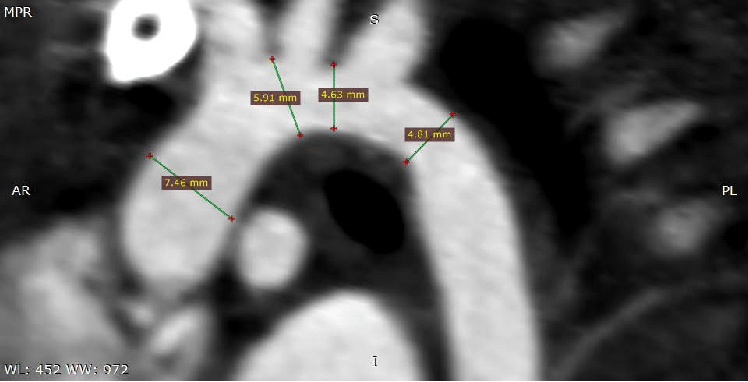
\includegraphics[width=0.8\textwidth]{figures/Conclusion/Ascending-aorta-aortic-arch-and-isthmic-region-in-a-double-oblique-plane-in-a.png}}
    \caption[Aorta Double Oblique Plane]{Aorta Double Oblique Plane}
    \label{fig_oblique}
\end{figure}

Successfully applying this algorithm will eliminate the need of verifying the segmentation result, discussed in Section \ref{stopping_condition}.

\subsection{Assurance Case}

There is room for improvements on the arguments of the requirements of \progname{}. The scope of our project was to explore the breadth of the work needed for an AC. The next step would be to go into the depth where necessary. The correctness of the document is reviewed and approved by a domain expert, where there should be evidences that can support the argument. The evidence for  E\_GA.1 discussed in Figure~\ref{fig_agr_ac_ga} is missing because we did not have the time to complete our Verification and Validation Plan (VnV). The VnV should include the test report, an evidence for E\_GA.1, that will indicate if \progname{} throws an exception when the inputs do not meet one or more of the assumptions, with a message that clearly states the reason.